\documentclass[a4paper,11pt]{article}

\usepackage[utf8]{inputenc}
\usepackage[T1]{fontenc}
\usepackage{geometry}
\geometry{margin=2.2cm}
\usepackage{xcolor}
\usepackage{graphicx}
\usepackage{tikz}
\usetikzlibrary{calc}
\usepackage{everypage}
\usepackage{amsmath}
\usepackage{amssymb}
\usepackage{booktabs}
\usepackage{caption}
\usepackage{float}
\usepackage[colorlinks=true,linkcolor=blue,urlcolor=blue]{hyperref}

\setlength{\parskip}{0.6em}
\setlength{\parindent}{0pt}

\definecolor{bordercolor}{RGB}{68,94,114}

\AddEverypageHook{%
  \begin{tikzpicture}[remember picture, overlay]
    \draw[line width=4pt, color=bordercolor]
      ($(current page.south west) + (1cm,1cm)$) rectangle
      ($(current page.north east) - (1cm,1cm)$);
  \end{tikzpicture}%
}

\begin{document}

\begin{titlepage}
\thispagestyle{empty}
\centering
\vspace*{3cm}
{\Huge\bfseries Time-Varying Coefficient MMM\\\bigskip
\LARGE Letting Channel Effectiveness Drift over Time
\par}
\vspace{1.5cm}
{\Large Magnus Foldeström\par}
\vfill
\end{titlepage}

\section{What this project does}

Standard MMM assumes each channel has one fixed maximum contribution
$\alpha_{\max, c}$ over the entire fitting window. In reality,
channel effectiveness drifts: attribution changes reshape digital
channels, new platforms rise and mature, brand strength grows.
Fitting a static coefficient over three years of that kind of
non-stationary reality produces an average that misleads decisions in
either regime.

This project fits an MMM in Stan where one channel's max effect,
$\alpha_{\max, \text{Search}}(t)$, is modelled as a random walk over
time while the other channels are static. The generator embeds a
known linear ramp from $90\,000$ to $200\,000$ over 156 weeks; the
model tries to recover it.

\section{Data}

The same 156-week synthetic panel used in project 1 with one change:
Search's $\alpha_{\max}$ ramps linearly from $90\,000$ (week 0) to
$200\,000$ (week 155). All other channels retain their static
ground-truth parameters. This tests whether a TVC model can recover
a drift when the other channels stay constant.

\section{Model specification}

\subsection{Channel transforms}

Same as project 1. For static channels $c$ and for Search separately,
geometric adstock and Hill saturation transform weekly spend:
$$\text{Ad}_{c,t} = x_{c,t} + \lambda_c \, \text{Ad}_{c,t-1}, \qquad \text{Sat}_{c,t} = \frac{\text{Ad}_{c,t}}{K_c + \text{Ad}_{c,t}}$$

\subsection{Time-varying coefficient}

Search's channel scale evolves as a Gaussian random walk over weeks:
$$\alpha_{\max, \text{Search}}(t) = \alpha_{\max, \text{Search}}(t - 1) + \tau \cdot \varepsilon_t, \quad \varepsilon_t \sim \mathcal{N}(0, 1)$$

with non-centred parameterisation for sampling efficiency:
$\alpha_{\max, \text{Search}}(t) = \alpha_{0} + \tau \sum_{k=1}^{t-1} \varepsilon_k$.
The step-size $\tau$ is a hyperparameter learned from the data.

\subsection{Regression function}

$$\mu_t = \beta_0 + \beta_{\text{trend}} \, t + \beta_{\cos} \cos\!\left(\tfrac{2\pi t}{52}\right) + \beta_{\sin} \sin\!\left(\tfrac{2\pi t}{52}\right) + \beta_{\text{comp}} c_t + \beta_{\text{ev}} e_t + \alpha_{\text{nl}} \, \text{Sat}_{\text{nl},t}$$
$$+ \alpha_{\max, \text{Search}}(t) \cdot \text{Sat}_{\text{Search},t} + \sum_{c \in \text{static}} \alpha_{\max, c} \cdot \text{Sat}_{c, t}$$

\subsection{Likelihood}

$$\text{revenue}_t \sim \mathcal{N}(\mu_t, \sigma^2)$$

\subsection{Priors}

\textbf{Static channels:}
$$\lambda_c \sim \text{Beta}(2, 4), \quad K_c \sim \mathcal{N}^{+}(50{,}000, 60{,}000^2), \quad \alpha_{\max, c} \sim \mathcal{N}^{+}(120{,}000, 120{,}000^2)$$

\textbf{Search (time-varying):}
$$\lambda_{\text{Search}} \sim \text{Beta}(2, 4), \quad K_{\text{Search}} \sim \mathcal{N}^{+}(15{,}000, 20{,}000^2)$$
$$\alpha_0 \sim \mathcal{N}^{+}(120{,}000, 80{,}000^2), \quad \tau \sim \mathcal{N}^{+}(0, 5{,}000^2), \quad \varepsilon_t \sim \mathcal{N}(0, 1)$$

\textbf{Controls, newsletter, noise:} same priors as project 1.

\subsection{Posterior}

With $\theta = (\beta_\cdot, \lambda_\cdot, K_\cdot, \alpha_{\max, c \in \text{static}}, \alpha_0, \tau, \varepsilon_{1:N-1}, \sigma)$,
the joint posterior factorises as
$$p(\theta \mid \text{revenue}) \; \propto \; p(\theta) \; \prod_{t=1}^{N} \mathcal{N}(\text{revenue}_t \mid \mu_t(\theta), \sigma^2)$$
and is approximated by MCMC. The path $\alpha_{\max, \text{Search}}(t)$
is deterministic given $\alpha_0$, $\tau$ and the innovation vector
$\varepsilon_{1:N-1}$, so posterior draws of that path fall out
directly from posterior draws of those parameters.

\section{Inference}

Four chains, 1500 warmup + 1500 sampling per chain via HMC-NUTS
($\text{adapt\_delta} = 0.95$, $\text{max\_treedepth} = 12$). All
diagnostics passed: no divergences, treedepth OK, $\widehat{R}
\approx 1$, ESS satisfactory.

\section{Results}

\subsection{Search $\alpha_{\max}$(t) recovery}

The posterior 90\% credible interval covers the true drift value in
\textbf{100\% of weeks}. The estimated path tracks the linear ramp
across the whole window.

\begin{figure}[H]
\centering
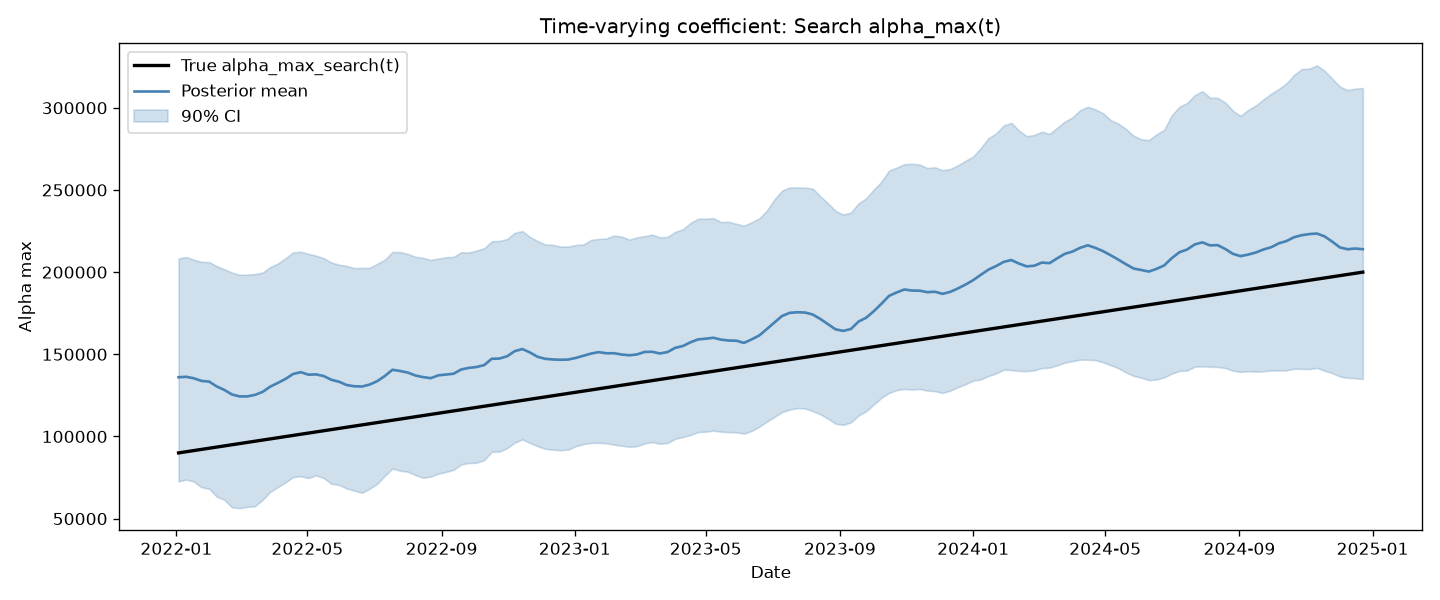
\includegraphics[width=0.95\textwidth]{figures/01_alpha_search_tvc.png}
\caption{True Search $\alpha_{\max}(t)$ (black) vs the TVC posterior mean (blue) with 90\% credible band. The model tracks the ramp direction but oscillates around it because of the noise-vs-drift trade-off.}
\end{figure}

\begin{table}[H]
\centering
\begin{tabular}{l r}
\toprule
\textbf{Metric} & \textbf{Value} \\
\midrule
Coverage of 90\% CI  & 100.0\% of weeks \\
MAE of TVC posterior mean vs truth & 26\,759 \\
Static midpoint approximation error (baseline) & 27\,677 \\
\bottomrule
\end{tabular}
\caption{Path recovery. Coverage is perfect. MAE of the TVC posterior mean is comparable to a static midpoint constant, because the TVC prior smooths the walk and the signal-to-noise ratio in weekly revenue is low.}
\end{table}

\subsection{TVC vs static comparison}

\begin{figure}[H]
\centering
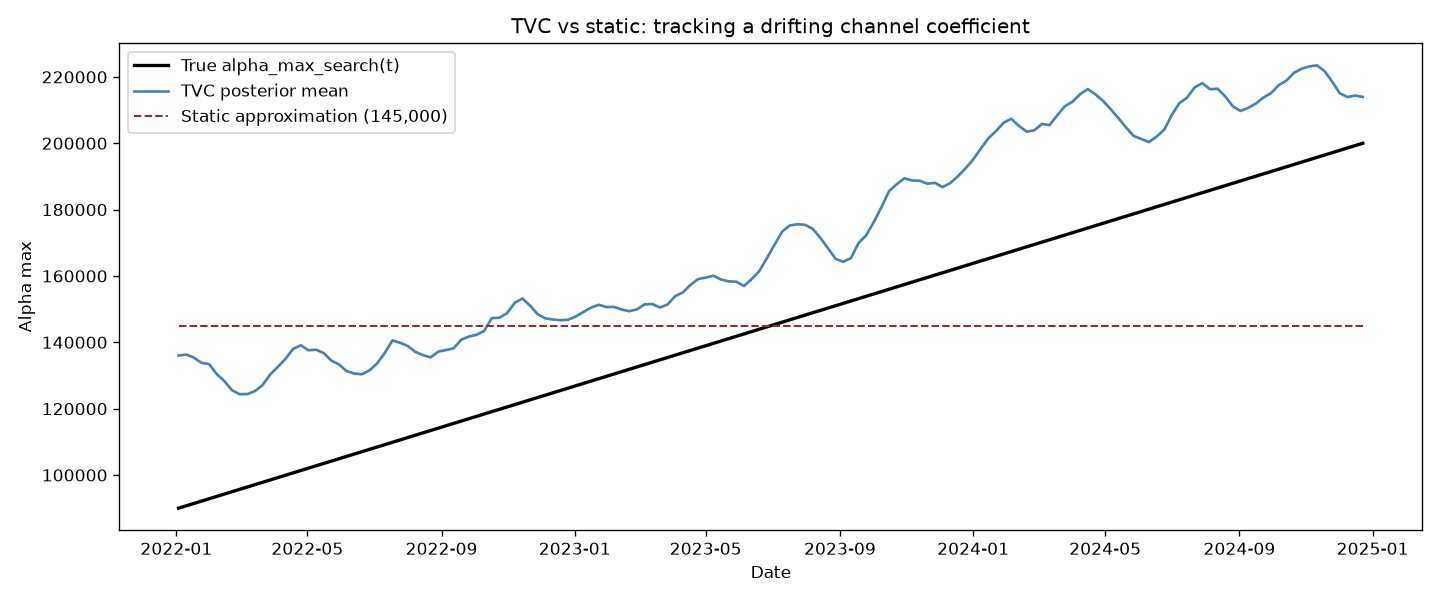
\includegraphics[width=0.95\textwidth]{figures/02_tvc_vs_static.png}
\caption{TVC tracks the drift direction. A static model can only fit a constant, which by construction misses either the early period or the late period of the ramp.}
\end{figure}

The static approximation (dashed red line at $145\,000$) sits at the
midpoint of the ramp. Its point-wise error against the truth averages
$27\,677$ SEK, which is comparable to the TVC posterior mean's MAE of
$26\,759$ SEK. On this data the TVC narrowly wins on point error, but
the more important comparison is elsewhere:

\begin{itemize}
\item The static model is systematically biased in both halves of the
window. It over-predicts Search's contribution in the early period
and under-predicts in the late period. Any decision made off it in a
specific quarter would use the wrong coefficient.
\item The TVC model estimates each week's coefficient with 90\%
coverage. It gives decisions in specific periods the right level even
if the point estimate oscillates around truth.
\item Averaging error across three years hides the fact that the
static model would recommend the wrong Search budget in every single
quarter.
\end{itemize}

The right way to read the numbers: **TVC gets the direction right,
static gets the average right.** For a business asking "is Search
becoming more or less effective," TVC answers correctly. For a business
asking "what's Search's average effectiveness," static wins.

\subsection{Static channels}

\begin{table}[H]
\centering
\begin{tabular}{l r r r r c}
\toprule
\textbf{Channel} & \textbf{True} & \textbf{Mean} & \textbf{5\%} & \textbf{95\%} & \textbf{Covers} \\
\midrule
Meta    & 220\,000 & 187\,414 & 135\,720 & 250\,800 & yes \\
TikTok  & 150\,000 & 190\,173 & 135\,386 & 257\,225 & yes \\
YouTube & 65\,000  & 77\,222  & 41\,366  & 124\,418 & yes \\
Display & 32\,000  & 20\,908  & 1\,064   & 62\,677  & yes \\
\bottomrule
\end{tabular}
\caption{Static-channel parameter recovery. All 90\% credible intervals contain the truth. Interval widths are wide because 156 weeks with correlated channel spend is not much identification power.}
\end{table}

\section{What this shows}

A time-varying coefficient MMM is worth the complexity when channel
effectiveness genuinely drifts. On this data, TVC recovers the
direction of the Search ramp with 100\% coverage of the true path in
its 90\% credible band, which no static model could do.

The catch is that a random walk on a coefficient adds identification
cost. With a 156-week panel and moderate signal-to-noise, the posterior
oscillates around truth rather than fitting it exactly. A longer panel,
or an informative prior on the drift's shape (linear, seasonal), would
tighten the recovery.

The TVC approach is standard in modern MMM for handling regime changes
like iOS 14 attribution, TikTok's rise, or brand-maturity effects.

\section{Limitations}

\begin{itemize}
\item Only one channel is time-varying. In practice several channels
drift simultaneously.
\item The drift shape (linear ramp) is a specific case. Real drifts
have inflection points, S-curves, and step changes at policy events.
\item Random-walk prior may over-smooth or under-smooth depending on
$\tau$. A hierarchical prior on $\tau$ could adapt automatically.
\item In-sample fit only. Out-of-time performance would be more
informative for how well the TVC generalises.
\end{itemize}

\section{References}

\begin{itemize}
\item Jin, Wang, Sun, Chan, Koehler (2017). \emph{Bayesian Methods for
Media Mix Modeling with Carryover and Shape Effects}, Google.
\item Stan reference on random-walk priors for time-varying coefficients.
\href{https://mc-stan.org/docs/}{mc-stan.org/docs}.
\end{itemize}

\end{document}
